
\chapter{Experiments}

\quad This chapter defined the experiments that are carried out as part of the laboratory. The first part was assigned to the presentation of the data set on which experiments have been made. All labels and the degree of correlation between them were explained. Second subchapter introduce to preprocessing process which was realized. Multi agent system and used learning strategy is demonstrated for each experiment in third subsection. The fourth chapter describes the implementation details: the technology used, the implementation of the multi-agent system and its mechanisms. The fifth section was devoted to the presentation of the results obtained. A number of charts and diagram descriptions have been included.


\section{Dataset information} 
The analysis dataset contains house sale prices for King County (includes also Seatlle), Washington in United States of America. Collected data constitute 21613 observations houses sold beetween May 2014 and May 2015.

\subsubsection{Labels in dataset}
Dataset consists of information of price, date of sale, id of sale and 18 house features. The below labels juxtaposition presents description of 18 parameters specify each property for sale:

\begin{description}
	\item[$\bullet$ house]- parameters which describe only house (apartment):	
	\begin{description}
		\item \textit{bedrooms} - number of bedrooms,
		\item \textit{bathrooms} - number of bathrooms, where 0.5 accounts for a room with a toilet but no shower,
		\item \textit{sqft\_living} - square footage of the apartments interior living space  ($m^2$),
		\item \textit{sqft\_living15} - living room area in 2015 (if the renovation was done in 2014-2015),
		\item \textit{floors} - total floors in house,
		\item \textit{view} - an index from 0 to 4 of how good the view of property was,
		\item \textit{condition} - an index from 1 to 5 on the overall condition of the apartment,
		\item \textit{grade} - an index from 1 to 13, where 1-3 falls short of building construction and design, 7 has an average level of construction and design, and 11-13 have a high quality level of construction and design,
		\item \textit{yr\_built} - the year of the house was initially built,
		\item \textit{yr\_renovated} - the year of the house last renovation,
	\end{description}
	\item[$\bullet$ property]- labels which specify property on sale:  
	\begin{description}
		\item \textit{sqft\_lot} - square footage of the land space,
		\item \textit{sqft\_lot15} - square footage of the land space in 2015,
		\item \textit{sqft\_above} - square footage of the interior housing space that is above ground level,
		\item \textit{sqft\_basement} - square footage of the interior housing space that is below ground level
	\end{description}
	\item[$\bullet$ location]- labels correlated with geographical location
	\begin{description}
		\item \textit{lat} - latitude (geographical coordinate), 
		\item \textit{lon} - longitude (geographical coordinates),
		\item \textit{zip\_code} - zip-code area the house is located, 
		\item \textit{waterfront} - if property has a waterfront view
	\end{description}
\end{description}

\subsubsection{Labels corellation}
\begin{center}
	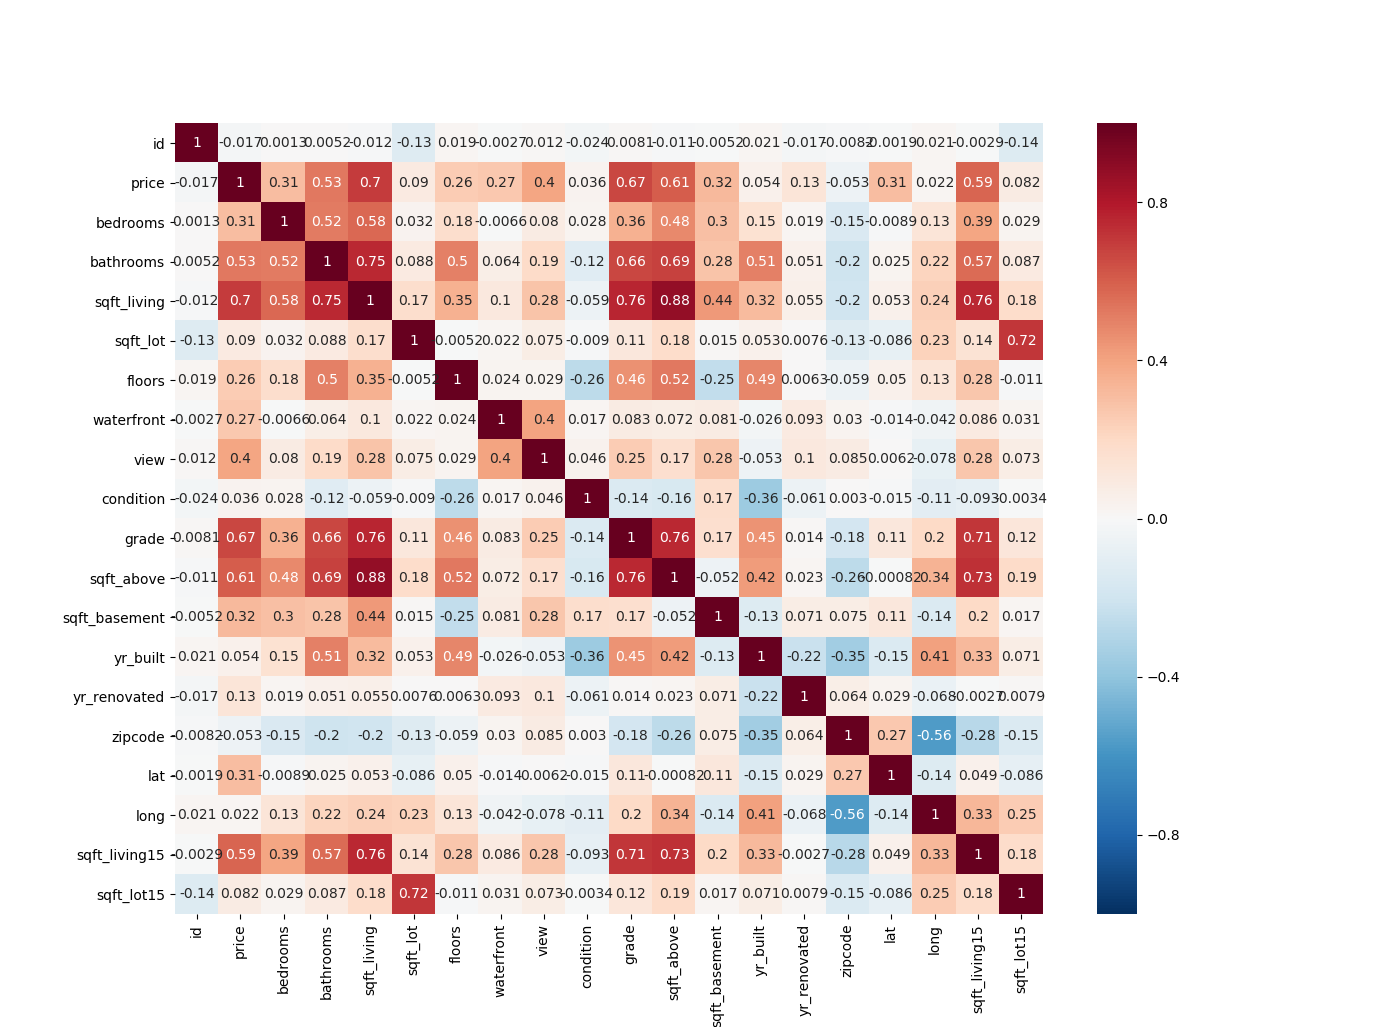
\includegraphics[width=1.2\textwidth, keepaspectratio]{diagrams/heatmap}
	\center
	\captionof{figure}{Heatmap presents corelation between labels.}
	\label{fig:heatmap}
\end{center}
\section{Data preprocessing} \label{sec:data-preprocessing}

%% https://www.slideshare.net/PawanShivhare1/predicting-king-county-house-prices
%% https://eu-gb.dataplatform.cloud.ibm.com/data/notebooks/converter/assets/f9c7a03e-250b-48a3-8188-e887f5f1213f?access_token=ad26bec15b3e6e34a44f7ce0724a103e766fd99f89a15d08a83654e775bea396&project=48fd3e84-65eb-4c78-83c0-d77ca776923f

\newpage
\section{Experiments definition}

\quad Agent configurations, environment and learning method has been described for each type of experiment. Experiment definition contains: \textit{Overview} (motivation), \textit{Description} and \textit{Schema}. Test instances differ from each other, among others, approach to learning, the agent's ability to observe the environment and specializations. There are two types of agents in this multi-agent system: Classifier Agent and Master Agent. The method of collecting results and communication between agents is similar for all established experiments. Communication is one-sided. Classifier agents only communicate with the master agent. Each regressor agent builds a training model based on which price prediction is created. The agent sends the created prediction model to the master agent. The master agent builds a general predictive model based on the received models from Classifier Agents.
\newline 
\quad The main outline of learning and data flow in this  system is described in the following diagram:
\newline
\begin{center}
	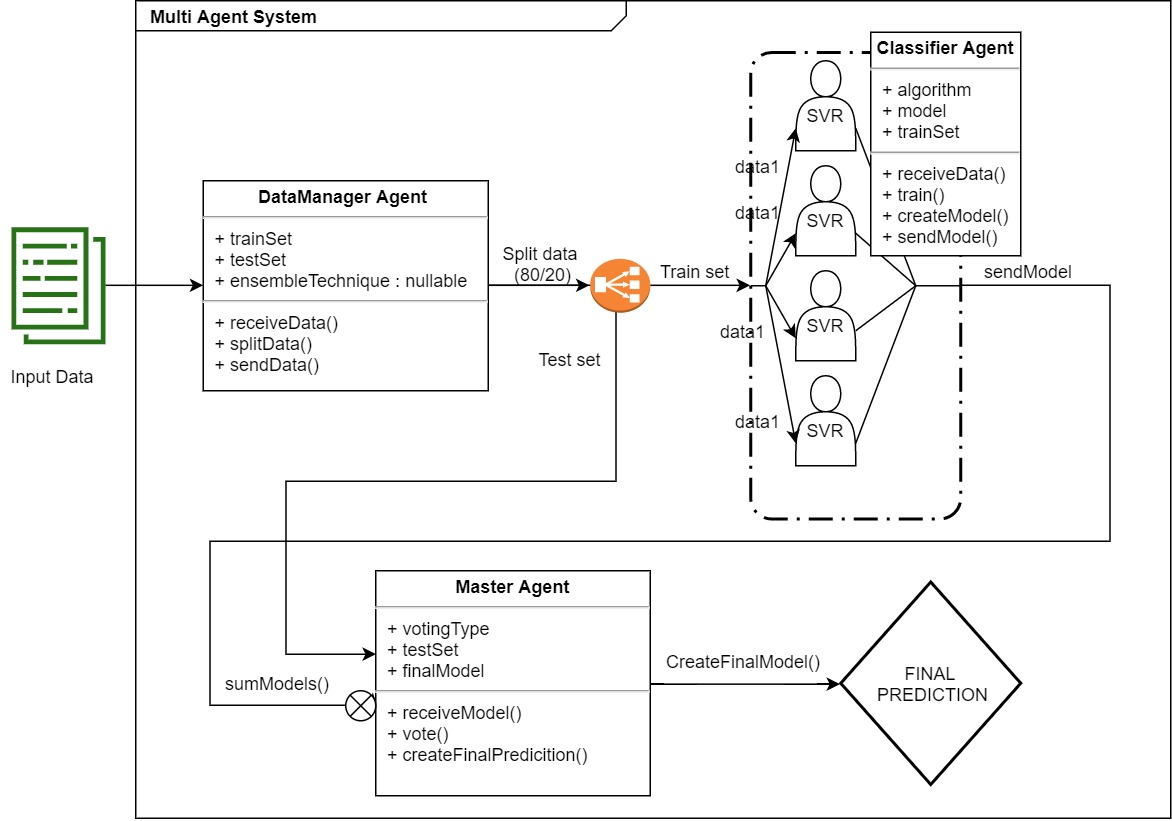
\includegraphics[width=0.9\textwidth, keepaspectratio]{diagrams/experiment1_schema.jpg}
	\center
	\captionof{figure}{The multi-agent system architecture where is presented data flow during classification process.}
	\label{fig:dataFlow}
\end{center}

% 1 eksperyment - gotowy
% zwykla populacja, te same klasyfikatory
% populacja mała

\newpage
\begin{enumerate}
	\item \textbf{Experiment}

\textit{Overview}
\newline
\quad The purpose of this experiment is to check how the multi-agent system works when each instance of classifier agents is learning from the same part of the data set. The visibility of agents who create a predictive model with the same classification algorithm is not limited. The population of agents in the system is not large (5 species), so as to check whether the potentially weak model created by a single agent can have a positive effect on the master agent final prediction.
\newline \newline
\textit{Description}
\begin{outline}[enumerate]
	\1 \textbf{Environment} \newline
	 In order to check the obtained predictive model in a multi-agent system, the environment is to be created by five instances of agents:
		\2 four classifier agents
		\2 one master agent
	\1 \textbf{Agents}
	\newline
	There are two types of agents in the system:
		\2 Classifier Agent - each agent implements the same machine learning algorithm. Agents has full information about the environment. Machine learning methods used as a part of this experiment:
			\3 Decision Tree Classifier
			\3 Support Vector Regressor (SVR)
			\3 K-Nearest Neighbours (K-NN)
			\3 Bayesian Ridge
		\2 Master Agent as a meta-classifier	 	
		
	\1 \textbf{Dataset}
	\newline
	The data set is splitted into training and test in the proportion of 80/20.
	Each Classifier Agent receives the same training set. The master agent uses the test set to classify the final predictive model.
	\1 \textbf{Final Prediciton}
	\newline
	The agent's master vote is done using the arithmetic average. The models are added together without rewarding potentially better predictive models.
\end{outline}

\textit{Schema}

\begin{center}
	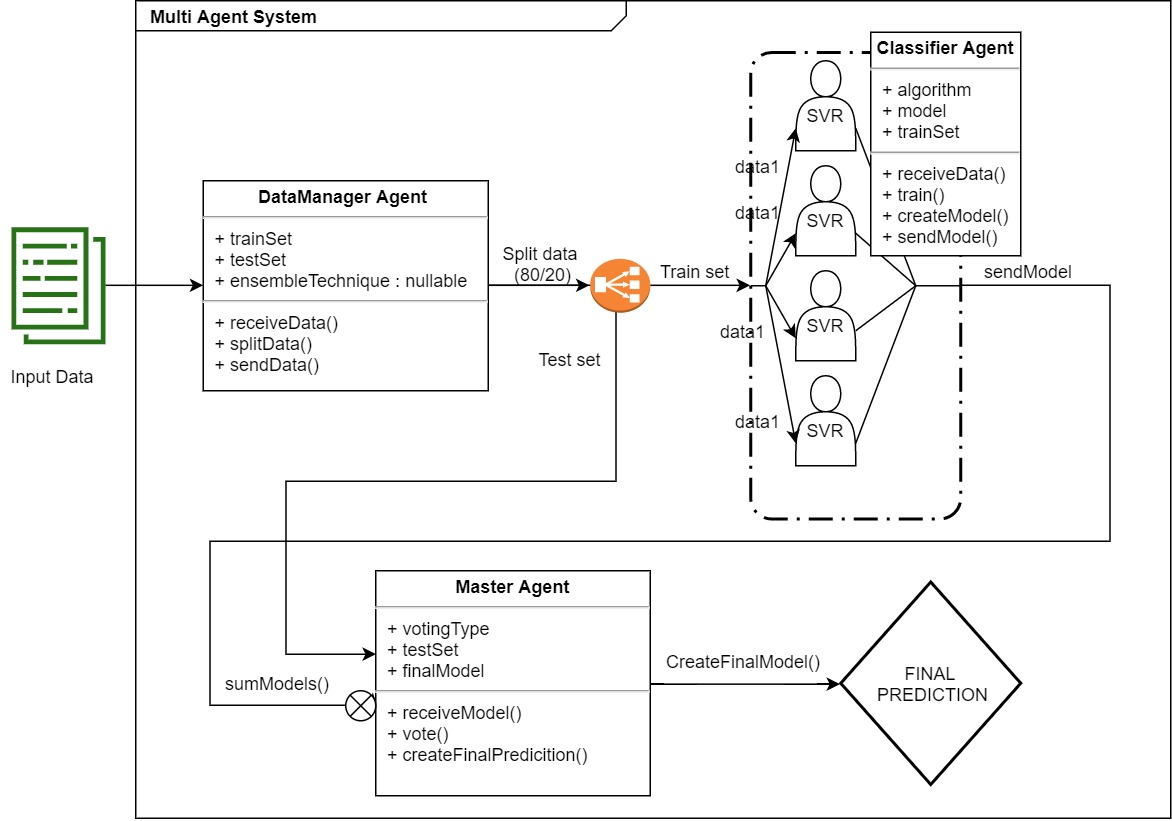
\includegraphics[width=1\textwidth, keepaspectratio]{diagrams/experiment1_schema.jpg}
	\center
    \captionof{figure}{Experiment 1 schema. Each Classifier Agent uses \emph{SVR} algorithm}
	\label{fig:exp1_schema}
\end{center}
%---------------------------------------

% 2 eksperyment - gotowy
% zwiekszona liczba agentów
% te same klasyfikatory

\newpage
\item 
\textbf{Experiment}

\textit{Overview}

The motivation to accomplish this experiment is to check the impact of the size of the population in the agent environment on the final predictive model. The number of models that are combined in the process of creating the concluding model is related to the size of the population in the agent system environment. Data distribution to agents, machine learning algorithms, and process of creation the final model by master agent are similar as it was described in experiment 1.
\newline \newline
\textit{Description}
\begin{outline}[enumerate]
	\1 \textbf{Environment} \newline
	The multi-agent system environment is implemented by a large number(9 species) of agents. The learning strategy is implemented by creating a model constructed by the artifacts of average sum of eight machine learning algorithms (methods are duplicated):
		\2 eight agents implementing machine learning algorithm
		\2 one master agent to create concluding decision
	\1 \textbf{Agents}
	\newline
	There are two types of agents in the system:
		\2 Classifier Agent - each agent implement the same machine learning algorithm. Agent observability of the environent is not limited. Machine learning methods used as a part of this experiment:
			\3 Decision Tree Classifier
			\3 Support Vector Regressor (SVR)
			\3 K-Nearest Neighbours (K-NN)
			\3 Bayesian Ridge
		\2 Master Agent as a meta-classifier	 	
	
	\1 \textbf{Dataset}
	\newline
	Each agent using the machine learning algorithm gets the same part of the data set (80\% of the entire set, 20\% is intended for the classification of the obtained results).
	\1 \textbf{Final Prediciton}
	\newline
	 The lead agent uses the weighted average method to create the final prediction model.
\end{outline}

\textit{Schema}
\begin{center}
	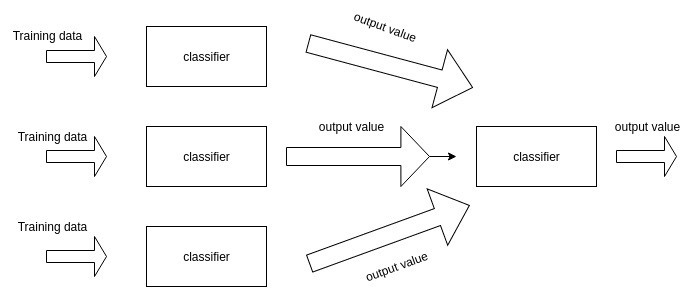
\includegraphics[width=1\textwidth, keepaspectratio]{diagrams/example.jpg}
	\center
	\captionof{figure}{Experiment 2 schema}
	\label{fig:exp1_schema}
\end{center}

%---------------------------------------

% 3 eksperyment - gotowy
% stacking - suma roznych klasyfikatorów
% populacja mała - suma roznyych (4 klasyfikatory agenci)

\newpage
\item 
\textbf{Experiment}

\textit{Overview}

\quad The motivation to conduct the experiment is to analyze the machine learning strategies used in the multi-agent system. The strategy being considered is stacking as an ensemble learning technique.The models will be created by agents which iplements different types of learning algorithms.
The impact of theoretically inferior models on the final solution will be contemplated.
\newline \newline
\textit{Description}
\begin{outline}[enumerate]
	\1 \textbf{Environment} \newline
	The multi-agent system environment is created by five species of agents. The learning strategy is implemented by creating a model constructed by the artifacts of four machine learning algorithms:
		\2 four agents implementing machine learning algorithm
		\2 one master agent to create concluding decision
	\1 \textbf{Agents}
	\newline
	There are two types of agents in the system:
		\2 Classifier Agent - each agent implement the same machine learning algorithm. Agent observability of the environent is not limited. Machine learning methods used as a part of this experiment:
			\3 Decision Tree Classifier
			\3 Support Vector Regressor (SVR)
			\3 K-Nearest Neighbours (K-NN)
			\3 Bayesian Ridge
	\2 Master Agent as a meta-classifier		
	
	\1 \textbf{Dataset}
	\newline
	Each agent using the machine learning algorithm gets the same part of the data set (80\% of the entire set, 20\% is intended for the classification of the obtained results).
	\1 \textbf{Final Prediciton}
	\newline
	The lead agent uses the weighted average method to create the final prediction model.
\end{outline}

\textit{Schema}

\begin{center}
	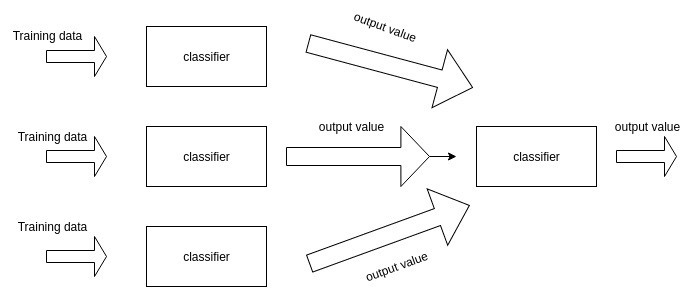
\includegraphics[width=1\textwidth, keepaspectratio]{diagrams/example.jpg}
	\center
	\captionof{figure}{Experiment 3 schema}
	\label{fig:exp1_schema}
\end{center}

% --- gotowe

% ----experiment 4

% -- Bagging & stacking
% -- najlepsze klasyfikatory

\newpage
\item 
\textbf{Experiment}


\textit{Overview}

The idea for which this experiment was performed is the use learning strategy which use ensemble learning techniques: bagging and stacking. The perception of individuals in the environment is limited due to the different part of the dataset obtained by the agents (bagging). However, agents have full knowledge of the data they received to make decisions when building the model. Only two types of classification algorithms are used to create ensemble model (stacking).
\newline \newline
\textit{Description}
\begin{outline}[enumerate]
	\1 \textbf{Environment} \newline
	Agents perception of the entire environment is limited. In multi-agent system enronment is created from:
		\2 four agents implementing machine learning algorithm
		\2 one master agent to create ensemble model
	\1 \textbf{Agents}
	\newline
	There are two types of agents in the system:
		\2 Classifier Agent - Each agent receive a different part of the training set (perception of the environment is limited).
		Agent implements one of the following classification algorithms:
			\3 Decision Tree Classifier
			\3 K-Nearest Neighbours (K-NN)
		\2 Master Agent as a meta-classifier	
	
	\1 \textbf{Dataset}
	\newline
	Data set has been evenly divided into five parts in the following proportions: 20:20:20:20:20. Four of the five parts will be used as training data and the last part will be used to classify final prediction model.
	\1 \textbf{Final Prediciton}
	\newline
	The single isntance of meta-classifier will use average voting when building the final model. Master agent assesses the built model on the last part of the divided data set.
\end{outline}

\textit{Schema}
\newline schemat

\begin{center}
	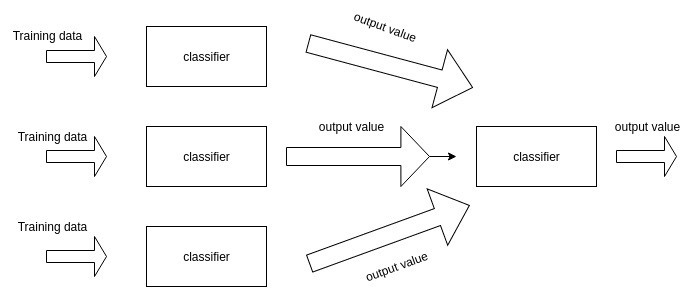
\includegraphics[width=1\textwidth, keepaspectratio]{diagrams/example.jpg}
	\center
	\captionof{figure}{Experiment 4 schema}
	\label{fig:exp1_schema}
\end{center}

% --- gotowe

% ----experiment 5
% trudniejsze srodowisko
% podzial na grupy eksperckie (agent ekspert w danym obszarze)
% grupy zformuowane na podstawie heatmapy

\newpage
\item 
\textbf{Experiment}
\newline
\textit{Overview}

The motivation in this experiment is to observe the decision making process when the agents cannot see the whole environment (partial observability). Agent-based environment is more difficult for each agent who create predictive model. Each agent will be an expert in a different area. 
Expert groups were formulated based on the correlation of labels (based on the heatmap). Every Classifier Agent implements a classification algorithm that builds a predictive model based on the labels defined in the group.
\newline \newline
\textit{Description}
\begin{outline}[enumerate]
	\1 \textbf{Environment} \newline
	The environment in multi-agent system is partially observable:
		\2 four agents where each is an expert in a given field (based on correlation beetwen labels):
			\3 specialization: bedrooms, bathrooms, sqft\_above, sqft\_living15
			\3 specialization: sqft\_living, sqft\_above, sqft\_living15, grade, sqft\_living15 
			\3 specialization: yr\_built, long, grade, floors, sqft\_living15 
			\3 specialization: zip code, longitude, latitude, yr\_renovated   
		\2 one master agent has no limitation of environment observability
	\1 \textbf{Agents}
	\newline
	There are two types of agents in the system:
	\2 Classifier Agent - each agent implements one of the following classification algorithm:
		\3 Decision Tree Classifier
		\3 K-nearest neighbours (K-NN)
	\2 Master Agent	as a meta-classifier	
	
	\1 \textbf{Dataset}
	\newline
	The data set is splitted 80/20 - 80\% of the entire set to train model(each agent the same part), 20\% is intended for the classification of the obtained results.
	\1 \textbf{Final Prediciton}
	\newline
	The master agent uses average voting to build the model predictive model
\end{outline}

\textit{Schema}
\newline schemat

\begin{center}
	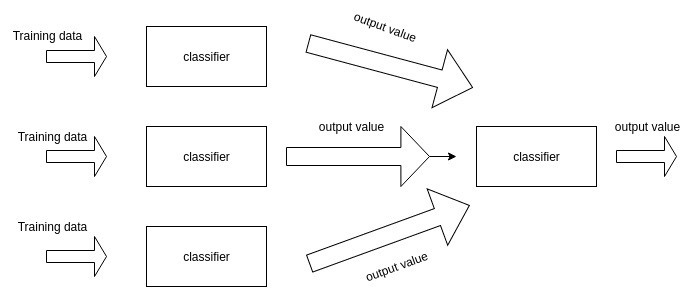
\includegraphics[width=1\textwidth, keepaspectratio]{diagrams/example.jpg}
	\center
	\captionof{figure}{Experiment 5 schema}
	\label{fig:exp1_schema}
\end{center}

% --- gotowe



% ----experiment 6
% trudniejsze srodowisko
% podzial na grupy eksperckie (agent ekspert w danym obszarze)
% grupy zformuowane wg mnie

\newpage
\item 
\textbf{Experiment}
o czym ma to być:
grupowanie po mojemu 

\textit{Overview}

The motivation to accomplish this the final model by master agent are similar as in Experiment 1.
\newline \newline
\textit{Description}
\begin{outline}[enumerate]
	\1 \textbf{Environment} \newline
	The multi-agent system constructed by the artifacts of average sum of sixteen machine learning algorithms (methods are duplicated):
	\2 fifteen agents implementing machine learning algorithm
	\2 one master agent to create concluding decision
	\1 \textbf{Agents}
	\newline
	There are two types of agents in the system:
	\2 Classifier Agent - each agent  of the environent is not limited. Machine learning methods used as a part of this experiment:
	\3 Decision Tree Classifier
	\3 Support Vector Regressor (SVR)
	\3 K-nearest neighbours (K-NN)
	\3 Bayesian Ridge
	\2 Master Agent		
	
	\1 \textbf{Dataset}
	\newline
	Each agent using the machine learning algorithm gets the same ssification of the obtained results).
	\1 \textbf{Final Prediciton}
	\newline
	The lead agent uses the weighted average method to create the final prediction model.
\end{outline}

\textit{Schema}
\newline schemat

\begin{center}
	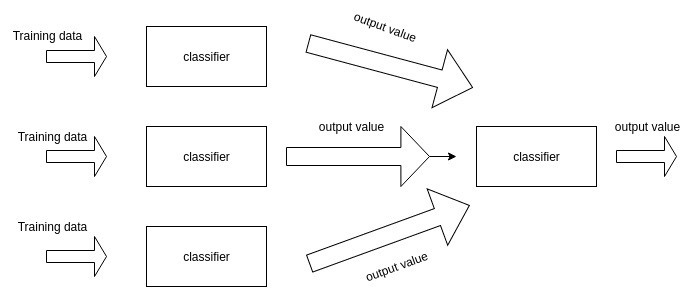
\includegraphics[width=1\textwidth, keepaspectratio]{diagrams/example.jpg}
	\center
	\captionof{figure}{Experiment 6 schema}
	\label{fig:exp1_schema}
\end{center}

% --- Bagging w grupowaniu po mojemu
% --- najlepsze typy klasyfiaktorów
%% chyba wtedy zbior treningowy bedzie za bardzo przebrany i nic z tego nie wyjdzie

Experymenty chapter
Konfiguracje agetnow + uczenia, podejście modelowe
Srodowisko uczynić trudniejszym, agent ni widzi całosci srodowiska (obserwowalnosc czesciowa)
Stwierdzic co sie dzieje jesli srodowisko nie jest obserwowalne (w pełni)
Specjalizacja, sensory etc
komunikacja agentów

	
\end{enumerate}

\section{Classification of the solution}

\section{Used technology}


\section{Results} \label{sec:api-detail}



